\subsection{How it works}

As said before, our algorithm first uses the Bron-Kerbosch algorithm to obtain
all the maximal cliques of the input graph. Then, it iterate through those maximal
cliques to looks for which cliques have the highest weight. \newline

\textbf{The Bron-Kerbosch pivot algorithm} that we use is a more efficient variant
of the initial algorithm. The basic form of the algorithm is inefficient in the
case of graphs with many non-maximal cliques as it makes a recursive call for
every clique, maximal or not. To save time and allow the algorithm to backtrack
more quickly in branches of the search that contain no maximal cliques, Bron and
Kerbosch introduced a variant of the algorithm involving a "pivot vertex". \newline

At each step, the algorithm keeps track of three groups of vertices: $R$ which is
a partially constructed (non-maximal) clique, $P$ which is the candidates vertices
that could be included in the clique and $X$ which is the excluded vertices that
already have been searched (because doing so would lead to a clique that has
already been found). The algorithm tries adding the candidate vertices one by one
to the partial clique, making a recursive call for each one. After trying each of
these vertices, it moves it to the set of vertices that should not be added again.
At each recursion, $P$ and $X$ are restricted to the neighbors of current vertex
being added to $R$ and when $P$ and $X$ are both empty there are no further
elements that can be added to $R$, $R$ is a maximal clique and the algorithm
reports $R$. \newline

The recursion is initiated by setting $R$ and $X$ to be the empty set and $P$ to
be the vertex set of the graph. Within each recursive call, the algorithm considers
the vertices $P$ in turn; if there a no such vertices, it either reports $R$ as
a maximal clique if $X$ is also empty, or continue. Then, a pivot vertex $u$ is
chosen from $P\cup X$ since any maximal clique must include either $u$ or one of
its non-neighbors, for otherwise the clique could be augmented by adding $u$ to it.
Only $u$ and its non-neighbors needs to be tested as the choices for the vertex
$v$ that is added to $R$ in each recusive call to the algorithm. For each vertex
$v$ chosen from $P\backslash N(u)$, with $N(u)$ being the neighbor set of $u$,
it makes a recursive call in which $v$ is added to $R$ and in which $P$ and $X$
are restriced to $N(v)$, which finds and reports all cliques extensions of $R$
that contains $v$. Then, it moves $v$ from $P$ to $X$ to exclude it from consideration
in future cliques and continues with the next vertex in $P\backslash N(u)$. \newline

To illustrate the Bron-Kerbosch algorithm, let's use the example in
Figure \ref{fig:basic-graph-example} on page \pageref{fig:basic-graph-example}:
\newline

\begin{minipage}{\linewidth}
    \textbf{Step 0:} \newline
    \begin{minipage}{0.4\textwidth}
        \begin{figure}[H]
            \centering
            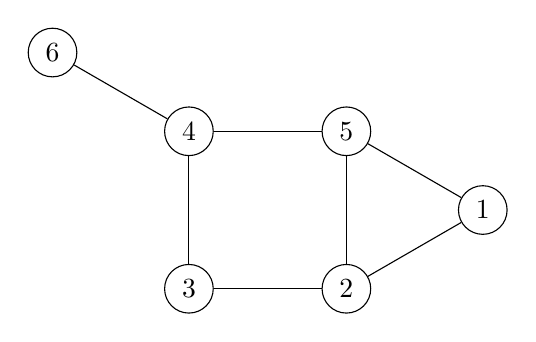
\begin{tikzpicture}[node distance=2cm, nodes={circle,draw}]
                \node (1) {1};
                \node (2) at ([shift=(210:2)] 1) {2};
                \node (3) [left of=2] {3};
                \node (4) [above of=3] {4};
                \node (5) [above of=2] {5};
                \node (6) at ([shift=(150:2)] 4) {6};

                \draw (1) -- (2);
                \draw (1) -- (5);
                \draw (2) -- (3);
                \draw (2) -- (5);
                \draw (3) -- (4);
                \draw (4) -- (5);
                \draw (4) -- (6);
            \end{tikzpicture}
            \caption{Graph illustration for the exact algorithm at step 0}
            \label{fig:exact-mewc-step0}
        \end{figure}
    \end{minipage}
    \begin{minipage}{0.6\textwidth}
        At the initial step, as said before, we will initialize $R$ and $X$ to be the
        empty set and $P$ to be the set of vertices of the graph.

        \begin{center}
            \begin{tabular}{|lll|}
                \hline
                R = \{\} & P = \{1,2,3,4,5,6\} & X = \{\} \\
                \hline
            \end{tabular}
        \end{center}
    \end{minipage}
\end{minipage} \newline

\begin{minipage}{\linewidth}
    \textbf{Step 1:} \newline
    \begin{minipage}{0.4\textwidth}
        \begin{figure}[H]
            \centering
            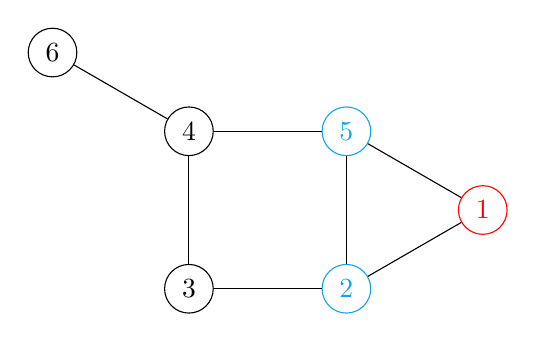
\begin{tikzpicture}[node distance=2cm, nodes={circle,draw}]
                \node[red] (1) {1};
                \node[Cerulean] (2) at ([shift=(210:2)] 1) {2};
                \node (3) [left of=2] {3};
                \node (4) [above of=3] {4};
                \node[Cerulean] (5) [above of=2] {5};
                \node (6) at ([shift=(150:2)] 4) {6};

                \draw (1) -- (2);
                \draw (1) -- (5);
                \draw (2) -- (3);
                \draw (2) -- (5);
                \draw (3) -- (4);
                \draw (4) -- (5);
                \draw (4) -- (6);
            \end{tikzpicture}
            \caption{Graph illustration for the exact algorithm at step 1}
            \label{fig:exact-mewc-step1}
        \end{figure}
    \end{minipage}
    \begin{minipage}{0.6\textwidth}
        In the first call of the function, since $P$ is not empty, we chose a
        pivot vertex $u$ in $P\cup X$. As it would be more time consuming to
        search for an appropriate pivot vertex, we simply chose the first one
        available, which will be represented in \textcolor{red}{red}. In this
        example we will always take the first element of $P$. The neighboring
        vertices of $u$ are represented in \textcolor{Cerulean}{blue}. \newline

        After that, we will iterate over the vertices of $P\backslash N(u)$,
        or in this case, $\{1,3,4,6\}$, and for each vertex $v$ we will make a
        recursive call to the function with $v$ added to $R$ and $P$ and $X$
        restricted to $N(v)$, which will find and report all cliques extensions
        of $R$ that contains $v$. \newline
    \end{minipage}
\end{minipage} \newline

\begin{minipage}{\linewidth}
    \textbf{Step 2:} \newline
    \begin{minipage}{0.4\textwidth}
        \begin{figure}[H]
            \centering
            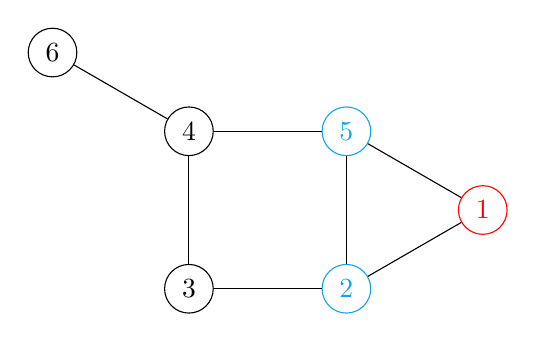
\begin{tikzpicture}[node distance=2cm, nodes={circle,draw}]
                \node[red] (1) {1};
                \node[Cerulean] (2) at ([shift=(210:2)] 1) {2};
                \node (3) [left of=2] {3};
                \node (4) [above of=3] {4};
                \node[Cerulean] (5) [above of=2] {5};
                \node (6) at ([shift=(150:2)] 4) {6};

                \draw (1) -- (2);
                \draw (1) -- (5);
                \draw (2) -- (3);
                \draw (2) -- (5);
                \draw (3) -- (4);
                \draw (4) -- (5);
                \draw (4) -- (6);
            \end{tikzpicture}
            \caption{Graph illustration for the exact algorithm at step 2}
            \label{fig:exact-mewc-step2}
        \end{figure}
    \end{minipage}
    \begin{minipage}{0.6\textwidth}
        At this step, since $P$ is not empty, we will choose a pivot vertex $u$
        in $P\cup X$. Here $u = 2$ and the algorithm will iterate over the
        vertices of $P\backslash N(u)$, which is $\{2\}$. \newline

        The next recursive call will be made with $P = \{5\}$, the pivot vertex
        will be $u = 5$ and then the next recusive call will report the clique
        $\{1,2,5\}$, which will be added to the list of cliques. \newline

        After that, the algorithm will backtrack to $R=\{\}$ since there will be
        no more iteration to do, and will add $1$ to $X$ as is was visited in
        its entirety. \newline

        The recursive call process looks like this:
        \begin{center}
            \begin{tabular}{|lll|}
                \hline
                R = \{1\}     & P = \{2,5\} & X = \{\} \\
                R = \{1,2\}   & P = \{5\}   & X = \{\} \\
                R = \{1,2,5\} & P = \{\}    & X = \{\} \\
                \hline
            \end{tabular}
        \end{center}
    \end{minipage}
\end{minipage} \newline

\begin{minipage}{\linewidth}
    \textbf{Step 3:} \newline
    \begin{minipage}{0.4\textwidth}
        \begin{figure}[H]
            \centering
            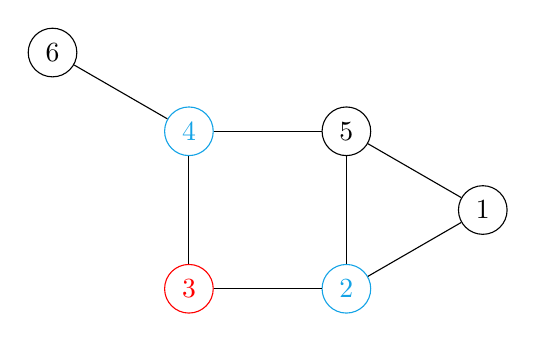
\begin{tikzpicture}[node distance=2cm, nodes={circle,draw}]
                \node (1) {1};
                \node[Cerulean] (2) at ([shift=(210:2)] 1) {2};
                \node[red] (3) [left of=2] {3};
                \node[Cerulean] (4) [above of=3] {4};
                \node (5) [above of=2] {5};
                \node (6) at ([shift=(150:2)] 4) {6};

                \draw (1) -- (2);
                \draw (1) -- (5);
                \draw (2) -- (3);
                \draw (2) -- (5);
                \draw (3) -- (4);
                \draw (4) -- (5);
                \draw (4) -- (6);
            \end{tikzpicture}
            \caption{Graph illustration for the exact algorithm at step 3}
            \label{fig:exact-mewc-step3}
        \end{figure}
    \end{minipage}
    \begin{minipage}{0.6\textwidth}
        At this step, since $P$ is not empty, we will choose a pivot vertex $u$
        in $P\cup X$. Here $u = 2$ and the algorithm will iterate over the
        vertices of $P\backslash N(u)$, which is $\{2,4\}$. \newline

        The next recursive calls will be made with $P = \{\}$ and $X = \{\}$, so
        they will report the cliques $\{2,3\}$ and $\{3,4\}$, which will be
        added to the list of cliques. \newline

        After that, the algorithm will backtrack to $R=\{\}$ since there will be
        no more iteration to do, and will add $3$ to $X$ as is was visited in
        its entirety. \newline

        The recursive call process looks like this:
        \begin{center}
            \begin{tabular}{|lll|}
                \hline
                R = \{3\}   & P = \{2,4\} & X = \{\} \\
                R = \{2,3\} & P = \{\}    & X = \{\} \\
                R = \{3,4\} & P = \{\}    & X = \{\} \\
                \hline
            \end{tabular}
        \end{center}
    \end{minipage}
\end{minipage} \newline

\begin{minipage}{\linewidth}
    \textbf{Step 4:} \newline
    \begin{minipage}{0.4\textwidth}
        \begin{figure}[H]
            \centering
            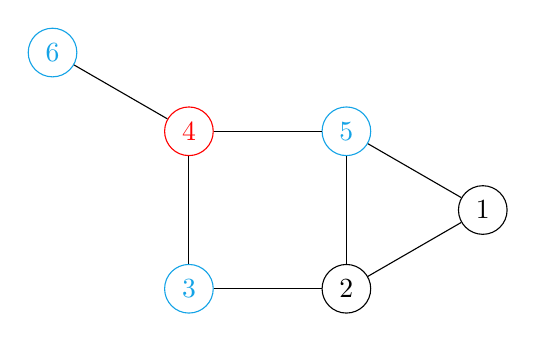
\begin{tikzpicture}[node distance=2cm, nodes={circle,draw}]
                \node (1) {1};
                \node (2) at ([shift=(210:2)] 1) {2};
                \node[Cerulean] (3) [left of=2] {3};
                \node[red] (4) [above of=3] {4};
                \node[Cerulean] (5) [above of=2] {5};
                \node[Cerulean] (6) at ([shift=(150:2)] 4) {6};

                \draw (1) -- (2);
                \draw (1) -- (5);
                \draw (2) -- (3);
                \draw (2) -- (5);
                \draw (3) -- (4);
                \draw (4) -- (5);
                \draw (4) -- (6);
            \end{tikzpicture}
            \caption{Graph illustration for the exact algorithm at step 4}
            \label{fig:exact-mewc-step4}
        \end{figure}
    \end{minipage}
    \begin{minipage}{0.6\textwidth}
        At this step, since $P$ is not empty, we will choose a pivot vertex $u$
        in $P\cup X$. Here $u = 3$ and the algorithm will iterate over the
        vertices of $P\backslash N(u)$, which is $\{5,6\}$. \newline

        The next recursive calls will be made with $P = \{\}$ and $X = \{\}$, so
        they will report the cliques $\{4,5\}$ and $\{4,6\}$, which will be
        added to the list of cliques. \newline

        After that, the algorithm will backtrack to $R=\{\}$ since there will be
        no more iteration to do, and will add $4$ to $X$ as is was visited in
        its entirety. \newline

        The recursive call process looks like this:
        \begin{center}
            \begin{tabular}{|lll|}
                \hline
                R = \{4\}   & P = \{5,6\} & X = \{3\} \\
                R = \{4,5\} & P = \{\}    & X = \{\}  \\
                R = \{4,6\} & P = \{\}    & X = \{\}  \\
                \hline
            \end{tabular}
        \end{center}
    \end{minipage}
\end{minipage} \newline

\begin{minipage}{\linewidth}
    \textbf{Step 5:} \newline
    \begin{minipage}{0.4\textwidth}
        \begin{figure}[H]
            \centering
            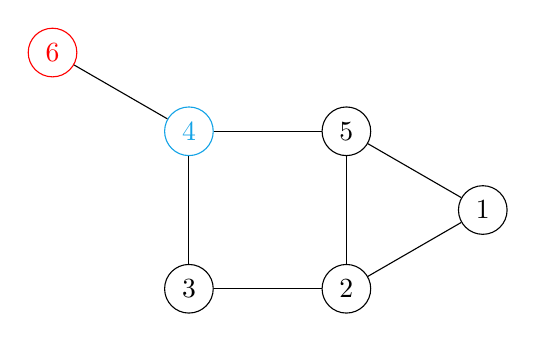
\begin{tikzpicture}[node distance=2cm, nodes={circle,draw}]
                \node (1) {1};
                \node (2) at ([shift=(210:2)] 1) {2};
                \node (3) [left of=2] {3};
                \node[Cerulean] (4) [above of=3] {4};
                \node (5) [above of=2] {5};
                \node[red] (6) at ([shift=(150:2)] 4) {6};

                \draw (1) -- (2);
                \draw (1) -- (5);
                \draw (2) -- (3);
                \draw (2) -- (5);
                \draw (3) -- (4);
                \draw (4) -- (5);
                \draw (4) -- (6);
            \end{tikzpicture}
            \caption{Graph illustration for the exact algorithm at step 5}
            \label{fig:exact-mewc-step5}
        \end{figure}
    \end{minipage}
    \begin{minipage}{0.6\textwidth}
        At this step, since $P$ is empty and $X$ is not, the algorithm will
        choose a pivot vertex $u$ in $X$. Here $u = 4$ but the algorithm will
        not be able to iterate further as $P\backslash N(4) = \{\}$. \newline

        The recursive call process looks like this:
        \begin{center}
            \begin{tabular}{|lll|}
                \hline
                R = \{6\} & P = \{\} & X = \{4\} \\
                \hline
            \end{tabular}
        \end{center}
    \end{minipage}
\end{minipage} \newline

The Bron-Kerbosch algorithm is now finished, and we have obtained the following
maximal cliques:
\begin{center}
    $\{(1,2,5),(2,3),(3,4),(4,5),(4,6)\}$
\end{center}

Now that we obtained the maximal cliques of the graph, we can compare them to find
the maximal edge-weighted clique. \newline

We will simply iterate over the maximal cliques and sum the weights of the edges
that are in the clique. The clique with the highest weight will be the maximal
edge-weighted clique. \newline

\begin{minipage}{\linewidth}
    If we want to explain everything in a more concise way, we can use the call
    process and tree of the algorithm.
    \begin{figure}[H]
        \centering
        \begin{tabular}{|l|}
            \hline
            BronKerbosch($\emptyset$, $\{1,2,3,4,5,6\}$, $\emptyset$)                           \\
            \hspace{1em} BronKerbosch(${1}$, $\{2,5\}$, $\emptyset$)                            \\
            \hspace{2em} BronKerbosch(${1,2}$, $\{5\}$, $\emptyset$)                            \\
            \hspace{3em} BronKerbosch(${1,2,5}$, $\emptyset$, $\emptyset$) : report $\{1,2,5\}$ \\
            \hspace{1em} BronKerbosch(${3}$, $\{2,4\}$, $\emptyset$)                            \\
            \hspace{2em} BronKerbosch(${2,3}$, $\emptyset$, $\emptyset$) : report $\{2,3\}$     \\
            \hspace{2em} BronKerbosch(${2,4}$, $\emptyset$, $\emptyset$) : report $\{2,4\}$     \\
            \hspace{1em} BronKerbosch(${4}$, $\{5,6\}$, ${3}$)                                  \\
            \hspace{2em} BronKerbosch(${4,5}$, $\emptyset$, $\emptyset$) : report $\{4,5\}$     \\
            \hspace{2em} BronKerbosch(${4,6}$, $\emptyset$, $\emptyset$) : report $\{4,6\}$     \\
            \hspace{1em} BronKerbosch(${6}$, $\emptyset$, ${4}$)                                \\
            \hline
        \end{tabular}
        \caption{Call process of the Bron-Kerbosch algorithm}
        \label{fig:call-process-bron-kerbosch}
    \end{figure}
    \begin{figure}[H]
        \centering
        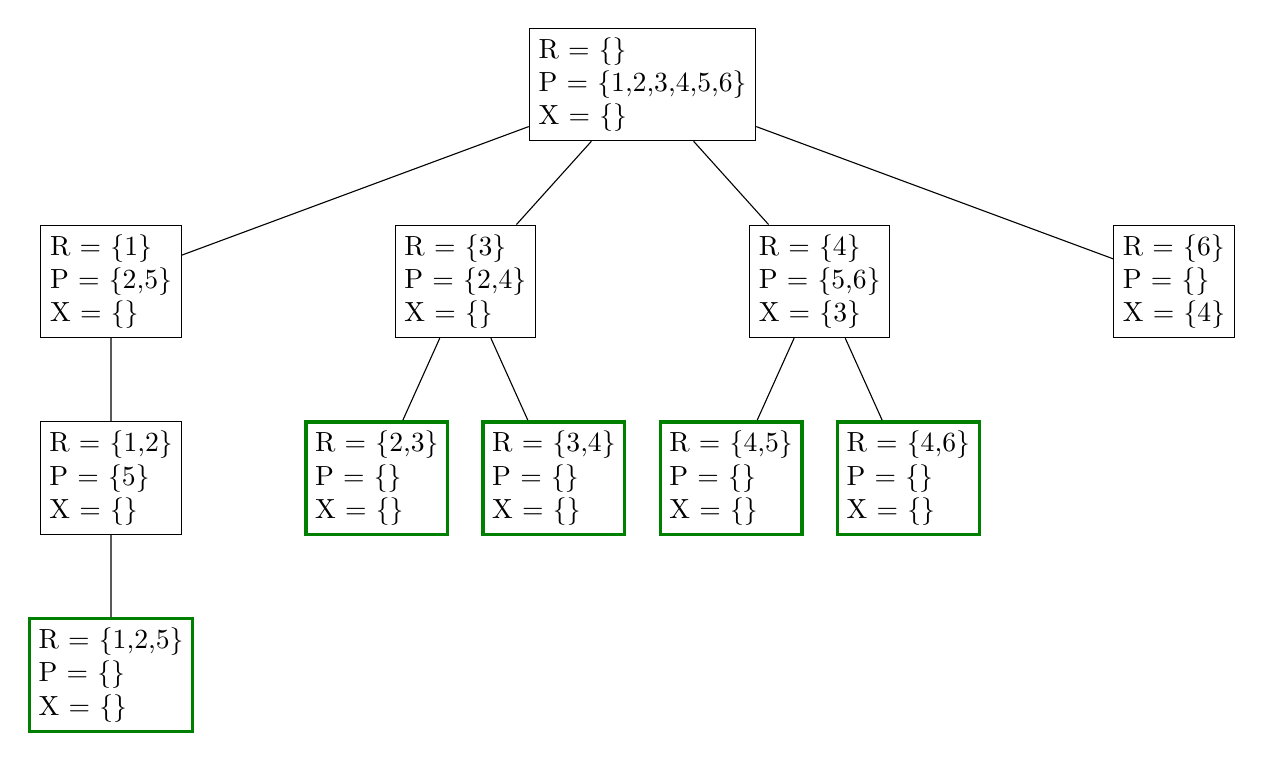
\begin{tikzpicture}[
                sibling distance=4.5cm,
                level distance=2.5cm,
                every node/.style={shape=rectangle, draw, align=left},
                level 2/.style={sibling distance=2.25cm}
            ]
            \node {
                R = \{\} \\
                P = \{1,2,3,4,5,6\} \\
                X = \{\}
            } child {
                    node {
                            R = \{1\} \\
                            P = \{2,5\} \\
                            X = \{\}
                        } child {
                            node {
                                    R = \{1,2\} \\
                                    P = \{5\} \\
                                    X = \{\}
                                } child {
                                    node[draw=Green, very thick] {
                                            R = \{1,2,5\} \\
                                            P = \{\} \\
                                            X = \{\}
                                        }}}}
            child {
                    node {
                            R = \{3\} \\
                            P = \{2,4\} \\
                            X = \{\}
                        } child {
                            node[draw=Green, very thick] {
                                    R = \{2,3\} \\
                                    P = \{\} \\
                                    X = \{\}
                                }}
                    child {
                            node[draw=Green, very thick] {
                                    R = \{3,4\} \\
                                    P = \{\} \\
                                    X = \{\}
                                }
                        }}
            child {
                    node {
                            R = \{4\} \\
                            P = \{5,6\} \\
                            X = \{3\}
                        } child {
                            node[draw=Green, very thick] {
                                    R = \{4,5\} \\
                                    P = \{\} \\
                                    X = \{\}
                                }}
                    child {
                            node[draw=Green, very thick] {
                                    R = \{4,6\} \\
                                    P = \{\} \\
                                    X = \{\}
                                }
                        }
                }
            child {
                    node {
                            R = \{6\} \\
                            P = \{\} \\
                            X = \{4\}
                        }
                };
        \end{tikzpicture}
        \caption{Call tree of the Bron-Kerbosch algorithm}
        \label{fig:call-tree-bron-kerbosch}
    \end{figure}
\end{minipage}